
%(BEGIN_QUESTION)
% Copyright 2012, Tony R. Kuphaldt, released under the Creative Commons Attribution License (v 1.0)
% This means you may do almost anything with this work of mine, so long as you give me proper credit

Identify which one of these opamp circuits is a {\it differentiator} versus which one is an {\it integrator}:

$$\includegraphics[width=15.5cm]{i01911x01.eps}$$

Next, write the equation (using calculus notation) for output voltage $y$ in terms of input voltage $x$ for the differentiator circuit:

\vskip 10pt

$y = $

\underbar{file i01911}
%(END_QUESTION)





%(BEGIN_ANSWER)

5 points for proper identification; 5 points for proper equation.  Deduct 2 points if the negative sign is missing from the equation.  Deduct 3 points if $RC$ is missing from the equation (i.e. something like $y = {dx \over dt}$).  Deduct 2 points if $\tau$ is written instead of $RC$):

$$\includegraphics[width=15.5cm]{i01911x02.eps}$$

$$y = -RC {dx \over dt}$$

%(END_ANSWER)





%(BEGIN_NOTES)

{\bf This question is intended for exams only and not worksheets!}.

%(END_NOTES)


